% Informe técnico final — Proyecto Integrador Kepler (APA 7 student paper)
\documentclass[a4paper,12pt]{article}
\usepackage[T1]{fontenc}
\usepackage[spanish]{babel}
\usepackage{lmodern}
\usepackage{setspace}
\usepackage[a4paper,top=2.54cm,bottom=2.54cm,left=2.54cm,right=2.54cm,
  headheight=14pt]{geometry}
\usepackage{indentfirst}
\usepackage{booktabs}
\usepackage{float}
\usepackage{graphicx}
\usepackage{caption}
\usepackage{fancyhdr}
\usepackage{titlesec}
\usepackage[hidelinks]{hyperref}
\usepackage{apacite}

% APA page layout: double spacing and a 1.27 cm indent on every paragraph.
\doublespacing
\setlength{\parindent}{1.27cm}
\setlength{\emergencystretch}{2em}

% APA heading levels 1-3.
\titleformat{\section}{\normalfont\bfseries\centering}{}{0pt}{}
\titleformat{\subsection}{\normalfont\bfseries}{}{0pt}{}
\titleformat{\subsubsection}{\normalfont\bfseries\itshape}{}{0pt}{}

% APA tables and figures: bold number, italic title above, note below.
\floatstyle{plaintop}\restylefloat{figure}
\captionsetup{position=top,labelsep=newline,labelfont=bf,textfont=it,
  justification=raggedright,singlelinecheck=false,skip=4pt}
\AtBeginDocument{\iflanguage{spanish}{\captionsetup[table]{name=Tabla}}{}}

% APA page header: page number at the top right.
\pagestyle{fancy}
\fancyhf{}
\rhead{\thepage}
\renewcommand{\headrulewidth}{0pt}

\renewcommand{\doiprefix}{https://doi.org/\ignorespaces}

\AtBeginDocument{%
  \renewcommand{\BOthers}{et al}%
  \renewcommand{\BOthersPeriod}{et al.}%
  \renewcommand{\BRetrievedFrom}{}%
  \renewcommand{\BRetrieved}[1]{}%
}

\begin{document}

  \begin{center}
    \vspace*{2cm}
    \textbf{Detección de candidatos a exoplaneta de la misión Kepler con
    aprendizaje automático: informe técnico final}
    \vspace{\baselineskip}

    Jheison Martinez Bolivar

    \vspace{\baselineskip}
    Facultad de Ingeniería, Universidad de La Salle

    Ciencia de Datos

    Docente de la asignatura Ciencia de Datos

    15 de noviembre de 2026
  \end{center}
  \newpage

  \begin{abstract}
    La misión Kepler detectó miles de señales de tránsito cuya verificación manual es
    costosa, por lo que clasificar automáticamente los objetos KOI marcados como
    candidatos es una pregunta abierta con salida práctica: producir una lista
    priorizada de candidatos a planeta. Este informe documenta el ciclo completo del
    proyecto: exploración del NASA Exoplanet Archive (9 564 KOI), limpieza con control
    de fuga de datos, tratamiento de valores faltantes no aleatorios, transformaciones
    logarítmicas e ingeniería de variables físicas; partición estratificada fija
    60/20/20 con métrica F1 macro; y comparación justa de un baseline de regresión
    logística contra bosques aleatorios, gradient boosting y SVM de núcleo RBF,
    afinados con RandomizedSearchCV y evaluados en prueba una sola vez. El modelo
    final de gradient boosting alcanzó F1 macro de 0.983 y AUC de 0.997 en prueba,
    frente a 0.946 y 0.991 del baseline, con 98.0 \% de los planetas recuperados y
    solo 24 errores de 1 518 objetos. La importancia por permutación muestra que el
    modelo aprende los mismos indicios físicos que usa el vetting astronómico
    (calidad de la señal y multiplicidad del sistema). Sobre los 1 977 candidatos sin
    verificar, el modelo propone 653 como planeta con probabilidad calibrada de
    decisión, priorizados en un entregable reproducible.
  \end{abstract}
  \newpage

  \section{Introducción y planteamiento del problema}

  La misión Kepler monitorizó cerca de 150 000 estrellas durante cuatro años para
  detectar caídas de brillo causadas por planetas que transitaban su estrella
  \cite{borucki2010}. El resultado del pipeline de detección es un catálogo de
  objetos de interés (KOI, por sus siglas en inglés), cada uno con una disposición:
  \textit{CONFIRMED} cuando el planeta está verificado, \textit{FALSE POSITIVE}
  cuando se demuestra que la señal es un eclipsamiento binario u otro artefacto, y
  \textit{CANDIDATE} cuando el objeto sigue sin resolver
  \cite{akeson2013}. Los 1 977 candidatos del catálogo acumulado representan
  trabajo de verificación pendiente para la comunidad: cada uno requeriría
  observaciones de seguimiento o análisis de vetting adicionales para confirmarse
  o descartarse \cite{thompson2018}.

  Este proyecto aborda ese problema como una tarea de clasificación binaria
  supervisada: aprender de los KOI ya resueltos (confirmados y falsos positivos)
  para estimar, para cada candidato, la probabilidad de que sea un planeta. La
  utilidad de un modelo así no está en sustituir el vetting astronómico, sino en
  \textbf{priorizar} la lista de candidatos: si el modelo asigna probabilidades
  coherentes con la física de los tránsitos, los casos con mayor probabilidad son
  los objetivos de seguimiento más prometedores.

  El proyecto se desarrolló como entrega final de la asignatura Ciencia de Datos en
  cuatro fases: diagnóstico exploratorio (NB1), limpieza e ingeniería de variables
  (NB2), modelo base y partición (NB3), comparación de modelos avanzados y
  elección del finalista (NB4), y visualizaciones más producto final (NB5). Todos
  los cuadernos están ejecutados de punta a punta en el repositorio entregado, de
  modo que cualquier cifra de este informe es reproducible con una sola pasada por
  el pipeline: CSV crudo $\rightarrow$ NB1 $\rightarrow$ NB2 $\rightarrow$ NB3
  $\rightarrow$ NB4 $\rightarrow$ NB5.

  \section{Datos y preparación}

  \subsection{Fuente y alcance}

  Los datos provienen del catálogo acumulado de KOI del NASA Exoplanet Archive
  \cite{akeson2013}, con 9 564 objetos y 153 columnas que mezclan parámetros
  astrofísicos (periodo orbital, radio, profundidad de tránsito, temperatura),
  diagnósticos de vetting estadístico y metadatos del pipeline. De ellos, 2 748
  están confirmados, 4 839 son falsos positivos y 1 977 permanecen como candidatos
  (Tabla~\ref{tab:inventario}). El conjunto etiquetado (7 587 objetos) alimenta el
  entrenamiento y la evaluación; los candidatos constituyen el conjunto de
  aplicación del producto final.

  \begin{table}[H]
    \caption{Inventario del conjunto de datos}
    \label{tab:inventario}
    \begin{tabular}{@{}lccc@{}}
      \toprule
      Subconjunto & Filas & Columnas & Uso en el proyecto \\
      \midrule
      CSV crudo & 9 564 & 153 & Punto de partida de NB1 \\
      Etiquetado (limpio) & 7 587 & 67 & Entrenamiento y evaluación \\
      \quad Planetas confirmados & 2 748 & --- & Clase positiva \\
      \quad Falsos positivos & 4 839 & --- & Clase negativa \\
      Candidatos (sin etiqueta) & 1 977 & 67 & Aplicación del modelo (NB5) \\
      \bottomrule
    \end{tabular}
    \par\medskip
    \begin{minipage}{\linewidth}
      \footnotesize\textit{Nota.} Las 67 columnas del conjunto limpio incluyen 66
      variables predictoras y la etiqueta binaria \texttt{es\_planeta}. El 36.2 \%
      del conjunto etiquetado son planetas.
    \end{minipage}
  \end{table}

  \subsection{Decisiones de limpieza e ingeniería (NB2)}

  La preparación fue la fase con mayor impacto sobre los resultados y se documentó
  en cuatro decisiones. Primera, el \textbf{descarte de columnas sin valor
  predictivo} en cuatro grupos: vacías o constantes; identificadores y metadatos
  (\texttt{kepoi\_name}, coordenadas, proveniencia); incertidumbres
  (\texttt{\_err1}/\texttt{\_err2}, que duplican la señal); y, sobre todo, las
  columnas de \textbf{fuga de datos}: \texttt{koi\_score},
  \texttt{koi\_pdisposition}, \texttt{kepler\_name}, las banderas
  \texttt{koi\_fpflag\_*} y los campos de veredicto del vetting. Esas columnas son
  el resultado del proceso que genera la etiqueta: incluirlas haría que el modelo
  acertara de forma casi perfecta en entrenamiento sin aprender nada útil para
  candidatos nuevos.

  Segunda, el \textbf{tratamiento de valores faltantes}. La mediana se calculó
  sobre las 63 columnas numéricas del conjunto etiquetado y se aplicó a las 57 con
  valores faltantes (robusta ante distribuciones astrofísicas fuertemente
  asimétricas), con las medianas guardadas en un JSON para reproducibilidad; ningún
  bloque superó el umbral de descarte del 70 \%. Esta imputación se calculó sobre el
  conjunto etiquetado completo, una fuga leve documentada cuyo efecto práctico es
  bajo (la mediana es robusta y el dataset es grande); el diseño de NB3 aísla la
  parte que sí importa: el escalado se ajusta solo con el bloque de entrenamiento
  dentro de cada pliegue. Lo relevante es que los nulos no son aleatorios
  (\textit{MNAR}): los bloques de diagnóstico donde la ausencia del dato predice
  casi determinísticamente la clase conservan información. Por eso se crearon
  indicadores binarios de ausencia por bloque (\texttt{na\_bloque\_tce},
  \texttt{na\_bloque\_vetting} y otros) antes de imputar, preservando esa señal en
  lugar de borrarla.

  Tercera, la \textbf{compresión de asimetría}: 34 variables con colas largas
  (radios, profundidades, conteos, señales) se transformaron con $\log(1+x)$, con
  lo que sus distribuciones quedaron comparables a una normal.

  Cuarta, la \textbf{ingeniería de variables físicas} en tres variables nuevas:
  \texttt{snr\_por\_transito} (calidad media de cada tránsito individual),
  \texttt{ratio\_dur\_periodo} (fracción del periodo que ocupa el tránsito, muy
  pequeña en órbitas rasantes) y \texttt{sistema\_multiple} (binario: el sistema
  tiene más de una señal). La multiplicidad es un criterio clásico del vetting:
  un sistema con varias señales coherentes es mucho más difícil de explicar con un
  eclipsamiento binario \cite{lissauer2012}, y se retomó en el diseño de la métrica
  de coherencia del producto final.

  \section{Metodología experimental}

  \subsection{Diseño de la evaluación (NB3)}

  La garantía de una comparación justa es el diseño antes que los modelos. La
  partición 60/20/20 estratificada se generó una vez con semilla fija (42) y se
  guardó en \texttt{koi\_splits.json}: 4 551 objetos de entrenamiento, 1 518 de
  validación y 1 518 de prueba, con la misma proporción de planetas en cada
  bloque. Todos los cuadernos cargan esa partición, así que ningún resultado
  depende de un corte afortunado.

  La métrica principal es el \textbf{F1 macro}, el promedio no ponderado del F1 de
  las dos clases. Con un 36.2 \% de positivos, la exactitud engaña: un modelo
  trivial que predice «falso positivo» siempre logra 63.8 \% de exactitud y F1
  macro de 0.389 (Tabla~\ref{tab:prueba}). El F1 macro penaliza esa asimetría
  porque exige desempeño igual en ambas clases, exactamente lo que interesa a un
  equipo que no quiere perder planetas raros.

  El baseline (NB3) combina dos referencias: un clasificador trivial por clase
  mayoritaria y una regresión logística dentro de un pipeline con
  \texttt{StandardScaler} y \texttt{class\_weight="balanced"}, que corrige el
  desbalance vía pesos de clase \cite{pedregosa2011}. El baseline alcanzó F1 macro
  de 0.946 en prueba, demostrando que la señal es aprendible y fijando el suelo
  que debían superar los modelos avanzados.

  \subsection{Modelos candidatos y búsqueda (NB4)}

  Se compararon tres familias que atacan el problema desde ángulos distintos:
  bosques aleatorios, que promedian árboles sobre muestras y variables aleatorias
  \cite{breiman2001}; gradient boosting con histogramas
  (\texttt{HistGradientBoostingClassifier}), la variante eficiente del boosting
  por gradiente \cite{ke2017}; y máquinas de soporte vectorial con núcleo RBF,
  capaces de fronteras no lineales en espacios de alta dimensión
  \cite{cortes1995}. Las tres admiten \texttt{class\_weight="balanced"} para el
  desbalance.

  La afinación se hizo con \texttt{RandomizedSearchCV}: 15 combinaciones
  aleatorias por familia sobre 5 pliegues estratificados (75 ajustes por familia),
  con la métrica F1 macro y \textbf{usando solo el bloque de entrenamiento}. La
  elección del ganador se tomó después con la validación intacta, y la prueba se
  evaluó una sola vez al final del proyecto. Para el SVM se usó la función de
  decisión durante la búsqueda (el AUC solo necesita orden) y la calibración de
  Platt se activó únicamente en el reentrenamiento final si el SVM ganaba; el
  ganador fue el gradient boosting, así que esa calibración no fue necesaria.

  El ganador se reentrenó con entrenamiento más validación (6 069 objetos) antes
  de la única evaluación en prueba, y sus hiperparámetros ganadores fueron:
  tasa de aprendizaje 0.06, 400 iteraciones, 63 hojas máximas, mínimo de 10
  muestras por hoja y regularización L2 nula. La interpretabilidad se obtuvo con
  importancia por permutación (15 barajados por variable sobre validación, con F1
  macro como objetivo) y el análisis de errores se centró en las dos direcciones
  del fallo: falsos planetas (falsos positivos marcados como planeta) y planetas
  perdidos.

  \begin{figure}[H]
    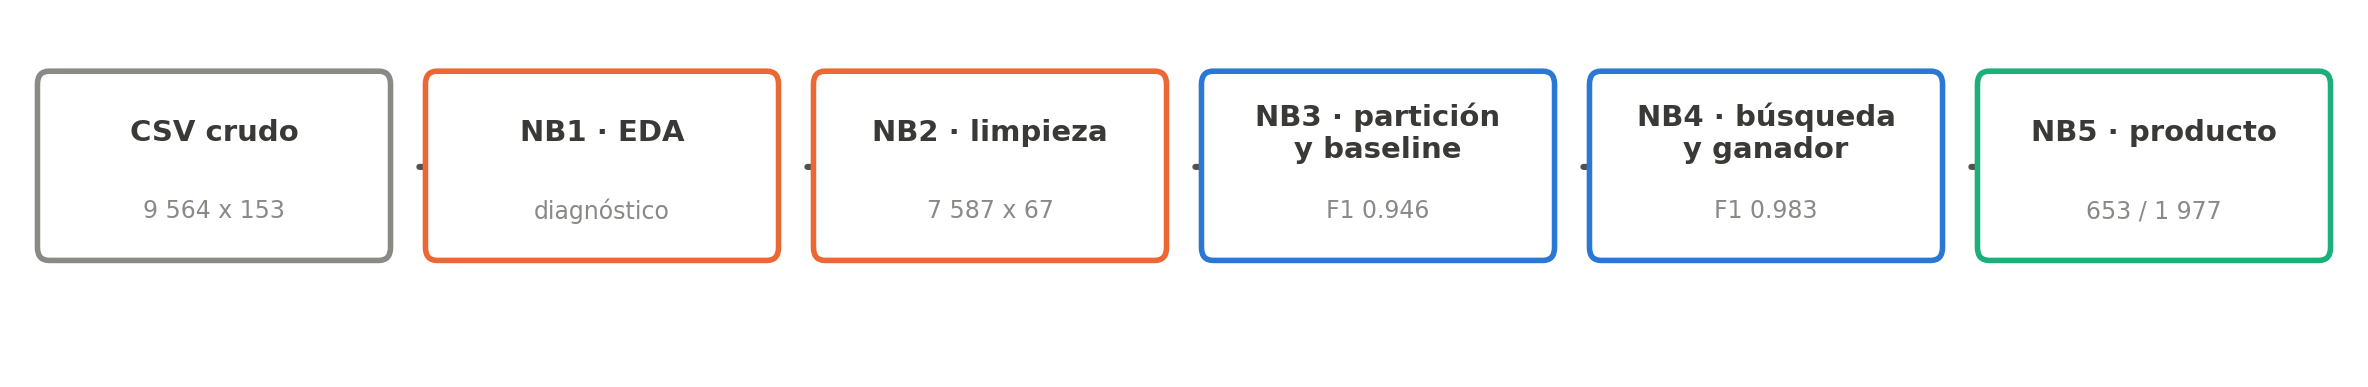
\includegraphics[width=\linewidth]{assets/images/fig-pipeline.png}
    \caption{Flujo completo del proyecto}
    \label{fig:pipeline}
    \par\medskip
    \begin{minipage}{\linewidth}
      \footnotesize\textit{Nota.} Cada bloque corresponde a un cuaderno ejecutado
      del repositorio; los artefactos intermedios (partición, métricas, modelo)
      se guardan en \texttt{data/} y se leen de nuevo en los cuadernos siguientes.
    \end{minipage}
  \end{figure}

  Todas las figuras de este informe se regeneraron a partir de los artefactos
  guardados del pipeline (métricas, partición, modelos y parquet de candidatos)
  con el script \texttt{render\_figs\_informe.py} incluido junto al informe, de
  modo que cada gráfico es reproducible sin re-entrenar nada.

  \section{Resultados}

  \subsection{Comparación de modelos}

  La Tabla~\ref{tab:comparacion} resume la competencia medida con la misma
  partición. Los tres modelos avanzados superan al baseline con claridad y el
  orden entre ellos es estrecho: el gradient boosting ganó por F1 macro en
  validación (0.982) con AUC de 0.997, seguido del bosque aleatorio (0.973) y del
  SVM (0.970). La Figura~\ref{fig:comparacion} muestra el mismo orden visualmente;
  la ventaja del ganador se mide sobre partición fija, de modo que es atribuible
  al modelo y no a la suerte del corte.

  \begin{table}[H]
    \caption{Comparación de los modelos en validación (bloque nunca usado en la búsqueda)}
    \label{tab:comparacion}
    \small
    \begin{tabular}{@{}lccc@{}}
      \toprule
      Modelo & F1 macro (CV) & F1 macro (validación) & AUC (validación) \\
      \midrule
      Baseline, reg. logística & 0.952 & 0.958 & 0.992 \\
      SVM, núcleo RBF & 0.962 & 0.970 & 0.996 \\
      Bosque aleatorio & 0.970 & 0.973 & 0.997 \\
      Gradient boosting (ganador) & 0.976 & 0.982 & 0.997 \\
      \bottomrule
    \end{tabular}
    \par\medskip
    \begin{minipage}{\linewidth}
      \footnotesize\textit{Nota.} CV = validación cruzada de 5 pliegues sobre el
      bloque de entrenamiento con la métrica F1 macro (la búsqueda usó 15
      iteraciones aleatorias por familia). La validación se usó una sola vez para
      elegir el ganador.
    \end{minipage}
  \end{table}

  \begin{figure}[H]
    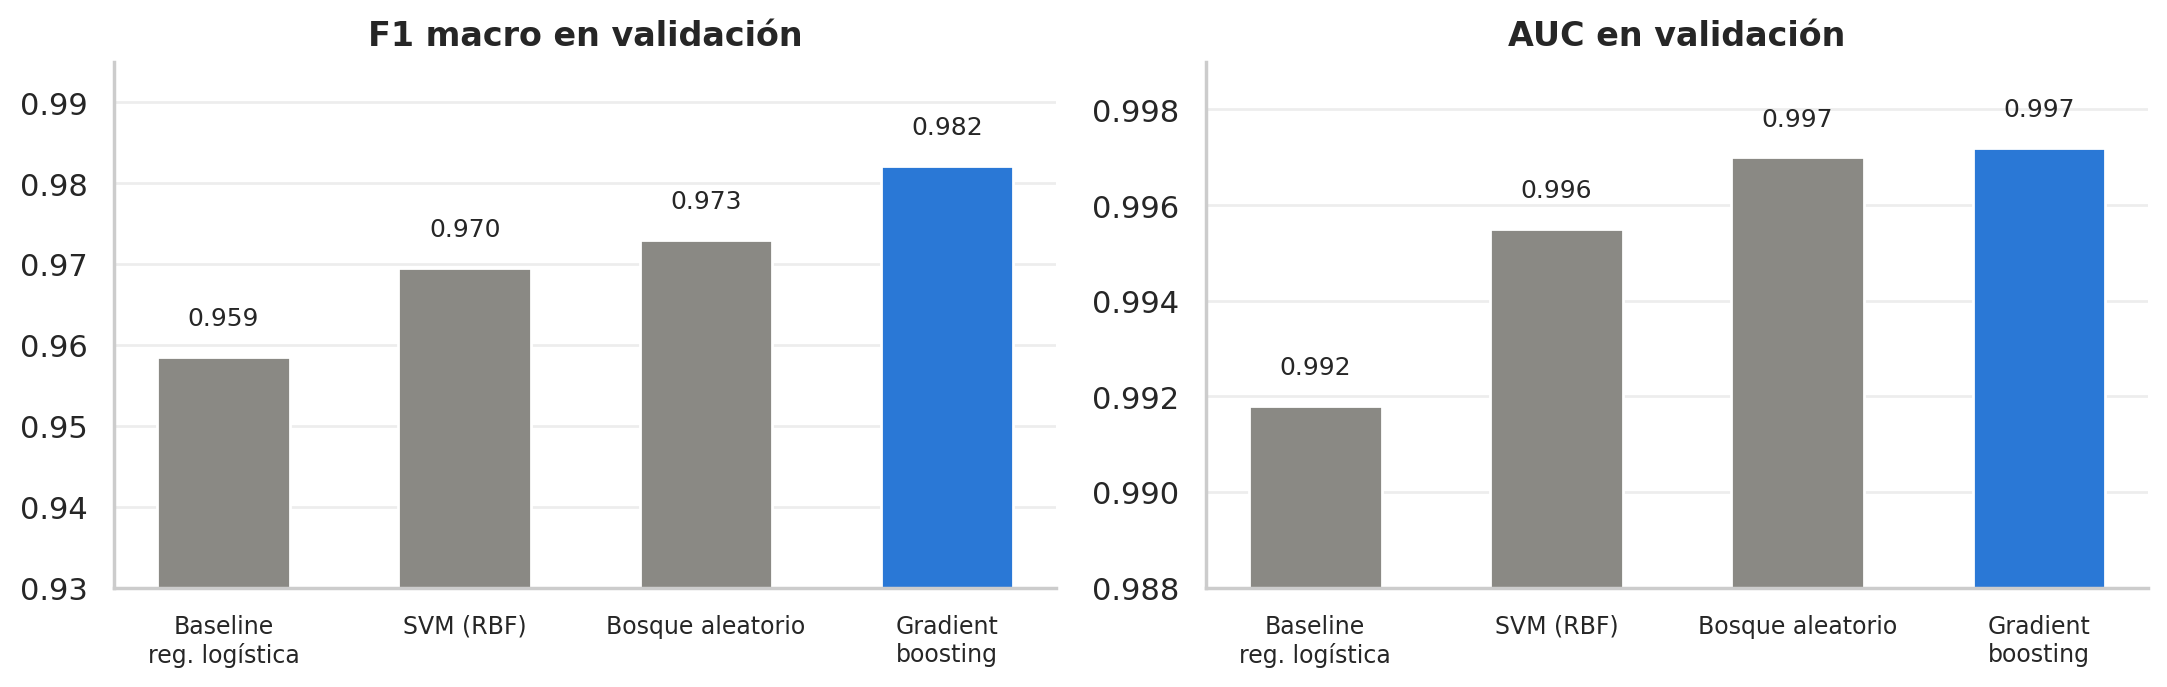
\includegraphics[width=\linewidth]{assets/images/fig-comparacion.png}
    \caption{F1 macro y AUC de los cuatro modelos en validación}
    \label{fig:comparacion}
    \par\medskip
    \begin{minipage}{\linewidth}
      \footnotesize\textit{Nota.} El ganador (azul) se define por F1 macro en
      validación; el AUC acompaña la decisión pero no la define.
    \end{minipage}
  \end{figure}

  \subsection{Evaluación final en prueba (una sola vez)}

  La Tabla~\ref{tab:prueba} y la Figura~\ref{fig:matriz} muestran el resultado del
  modelo final reentrenado en su único contacto con la prueba: F1 macro de 0.983
  (0.037 sobre el baseline) y AUC de 0.997. De los 550 planetas reales del bloque
  de prueba, el modelo recupera 539 (98.0 \% de sensibilidad); de los 968 falsos
  positivos, descarta bien 955 (98.7 \% de especificidad). Solo 24 objetos de
  1 518 quedan mal clasificados: 13 falsos planetas (alarmas que se examinarían a
  mano en el flujo real) y 11 planetas perdidos (pérdida real de descubrimiento).

  \begin{table}[H]
    \caption{Métricas en el bloque de prueba, tocado una sola vez}
    \label{tab:prueba}
    \begin{tabular}{@{}lccccc@{}}
      \toprule
      Modelo & Exactitud & Precisión & Sensibilidad & F1 macro & AUC \\
      \midrule
      Trivial (clase mayoritaria) & 0.638 & 0.000 & 0.000 & 0.389 & 0.500 \\
      Baseline, reg. logística & 0.950 & 0.909 & 0.958 & 0.946 & 0.991 \\
      Gradient boosting (final) & 0.984 & 0.976 & 0.980 & 0.983 & 0.997 \\
      \midrule
      $\Delta$ F1 macro frente al baseline & & & & +0.037 & \\
      \bottomrule
    \end{tabular}
    \par\medskip
    \begin{minipage}{\linewidth}
      \footnotesize\textit{Nota.} $n = 1 518$; 550 planetas y 968 falsos
      positivos. Precisión y sensibilidad se reportan sobre la clase planeta. El
      trivial predice siempre la clase mayoritaria, por eso su precisión y
      sensibilidad planetaria son nulas.
    \end{minipage}
  \end{table}

  \begin{figure}[H]
    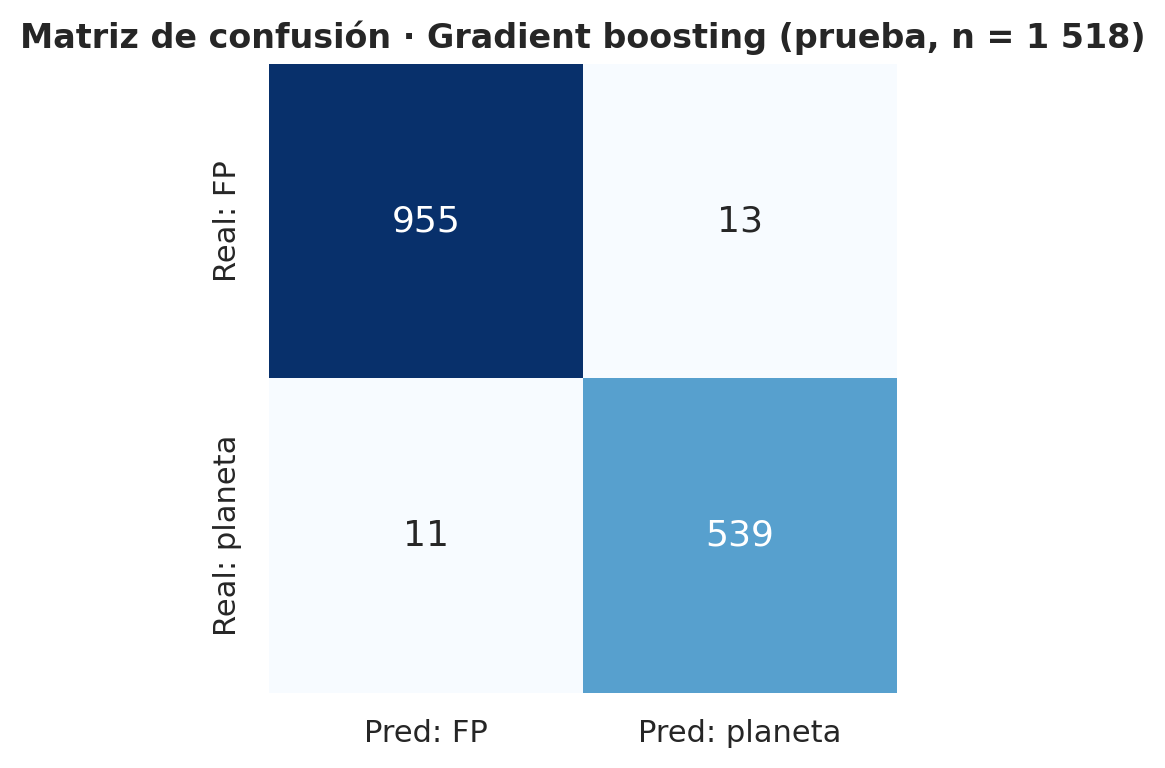
\includegraphics[width=0.5\linewidth]{assets/images/fig-matriz.png}
    \caption{Matriz de confusión del modelo final en prueba}
    \label{fig:matriz}
    \par\medskip
    \begin{minipage}{\linewidth}
      \footnotesize\textit{Nota.} Filas: clase real; columnas: predicción con
      umbral 0.5. Los 24 errores se analizan por dirección en el texto.
    \end{minipage}
  \end{figure}

  La curva ROC de la Figura~\ref{fig:roc} confirma la mejora: la curva del
  gradient boosting queda por encima del baseline en casi todo el rango, con la
  mayor separación en tasas bajas de falsos positivos, la zona que interesa en la
  práctica porque corresponde a listas de candidatos limpias.

  \begin{figure}[H]
    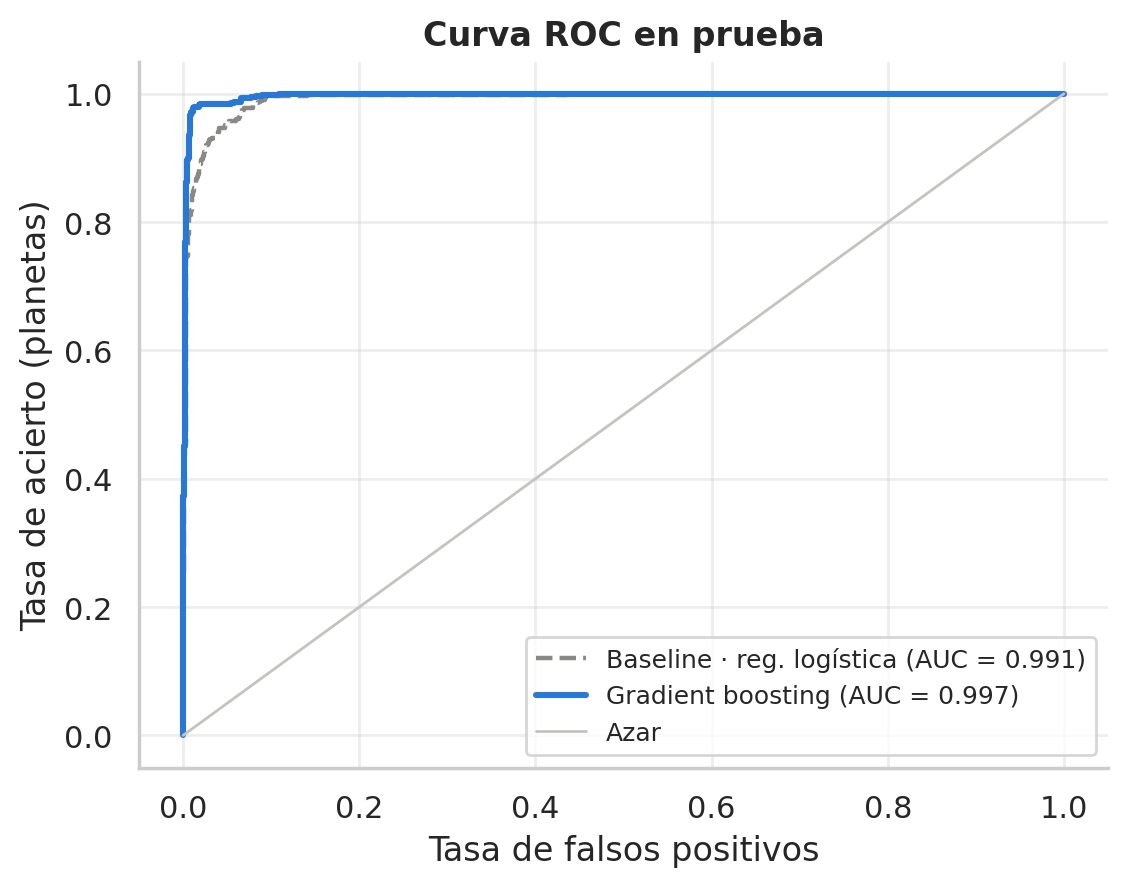
\includegraphics[width=0.55\linewidth]{assets/images/fig-roc.png}
    \caption{Curva ROC del modelo final frente al baseline en prueba}
    \label{fig:roc}
    \par\medskip
    \begin{minipage}{\linewidth}
      \footnotesize\textit{Nota.} La diagonal es el azar. A igual tasa de falsos
      positivos, el modelo final encuentra más planetas.
    \end{minipage}
  \end{figure}

  \subsection{Qué mira el modelo: importancia por permutación}

  La Figura~\ref{fig:importancia} muestra la caída del F1 macro al barajar cada
  variable en validación. El orden lo dominan la \textbf{calidad de la señal}
  (\texttt{log\_koi\_prad} con 0.084, \texttt{koi\_dikco\_msky} con 0.036,
  \texttt{log\_koi\_max\_mult\_ev} con 0.026) y los indicadores de ausencia MNAR
  (\texttt{na\_bloque\_tce} con 0.021), seguidos de las variables físicas
  construidas (\texttt{ratio\_dur\_periodo} con 0.023). La lectura física es
  directa: el modelo aprende los mismos indicios que usa el vetting astronómico,
  radios de tránsito verosímiles, contornos de foco de la señal coherentes y
  detección de eventos múltiples; y nada de esto se explica sin la limpieza, pues
  barajar las variables de calidad cuesta hasta 0.084 de F1 macro.

  \begin{figure}[H]
    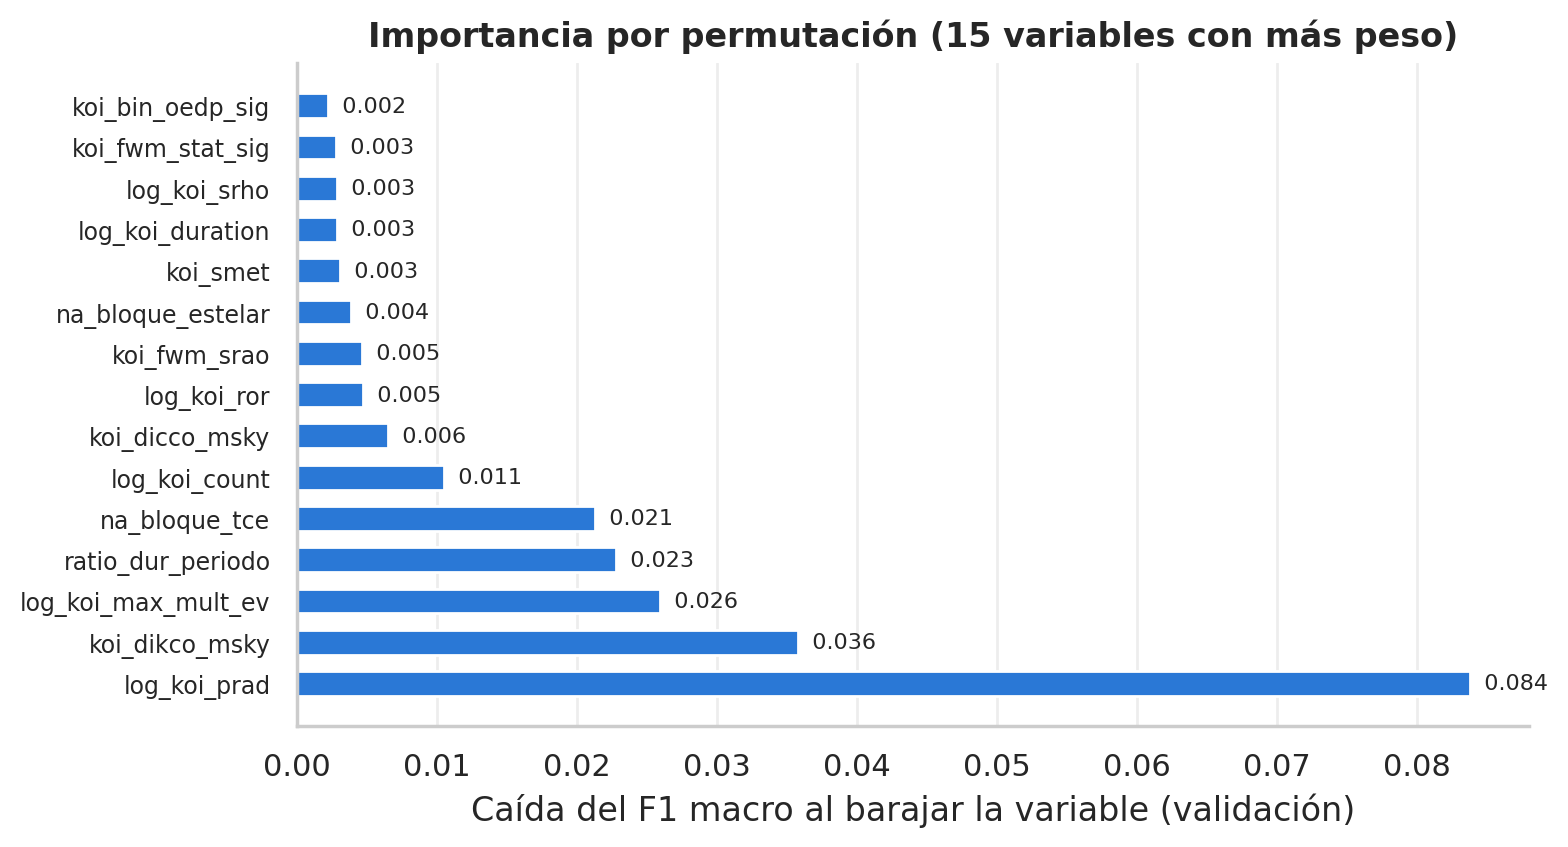
\includegraphics[width=\linewidth]{assets/images/fig-importancia.png}
    \caption{Importancia por permutación de las 15 variables con más peso}
    \label{fig:importancia}
    \par\medskip
    \begin{minipage}{\linewidth}
      \footnotesize\textit{Nota.} Caída media del F1 macro al barajar la variable
      (15 repeticiones, sobre validación). Prefijos \texttt{log\_}: variable
      transformada con $\log(1+x)$; \texttt{na\_bloque\_*}: indicador de ausencia
      MNAR.
    \end{minipage}
  \end{figure}

  El análisis de errores refuerza esa lectura. Los planetas perdidos se
  concentran en señales de baja relación señal-ruido o geometrías rasantes, con
  probabilidades predichas cerca del umbral; los falsos planetas son tránsitos
  profundos en sistemas pequeños, el nicho donde un eclipsamiento binario
  imita mejor a un planeta. En ambos casos el modelo duda cerca del umbral 0.5:
  los errores ocurren donde el problema es genuinamente ambiguo, no por fallas
  del pipeline de datos.

  \section{Producto final: clasificación de los 1 977 candidatos}

  El entregable práctico del proyecto es la clasificación de los candidatos
  guardada en \texttt{koi\_candidatos\_clasificados.parquet}: para cada uno, la
  probabilidad predicha de «planeta» y la decisión con umbral 0.5. La
  correspondencia fila a fila entre ese parquet y el CSV crudo queda verificada
  dentro del Notebook 5: además del conteo de candidatos, se comprueba que el
  periodo transformado del parquet ($\exp(\log(1+x))-1$) reproduce, fila a fila,
  el periodo crudo de cada candidato del catálogo. El modelo
  propone 653 de 1 977 como planeta (33.0 \%). El histograma de la
  Figura~\ref{fig:zonas} muestra decisiones mayoritariamente firmes: 607
  candidatos con probabilidad de al menos 0.75 y 1 278 con menos de 0.25; solo 92
  quedan en la zona gris intermedia, que es exactamente la cola candidata a
  revisión manual.

  \begin{figure}[H]
    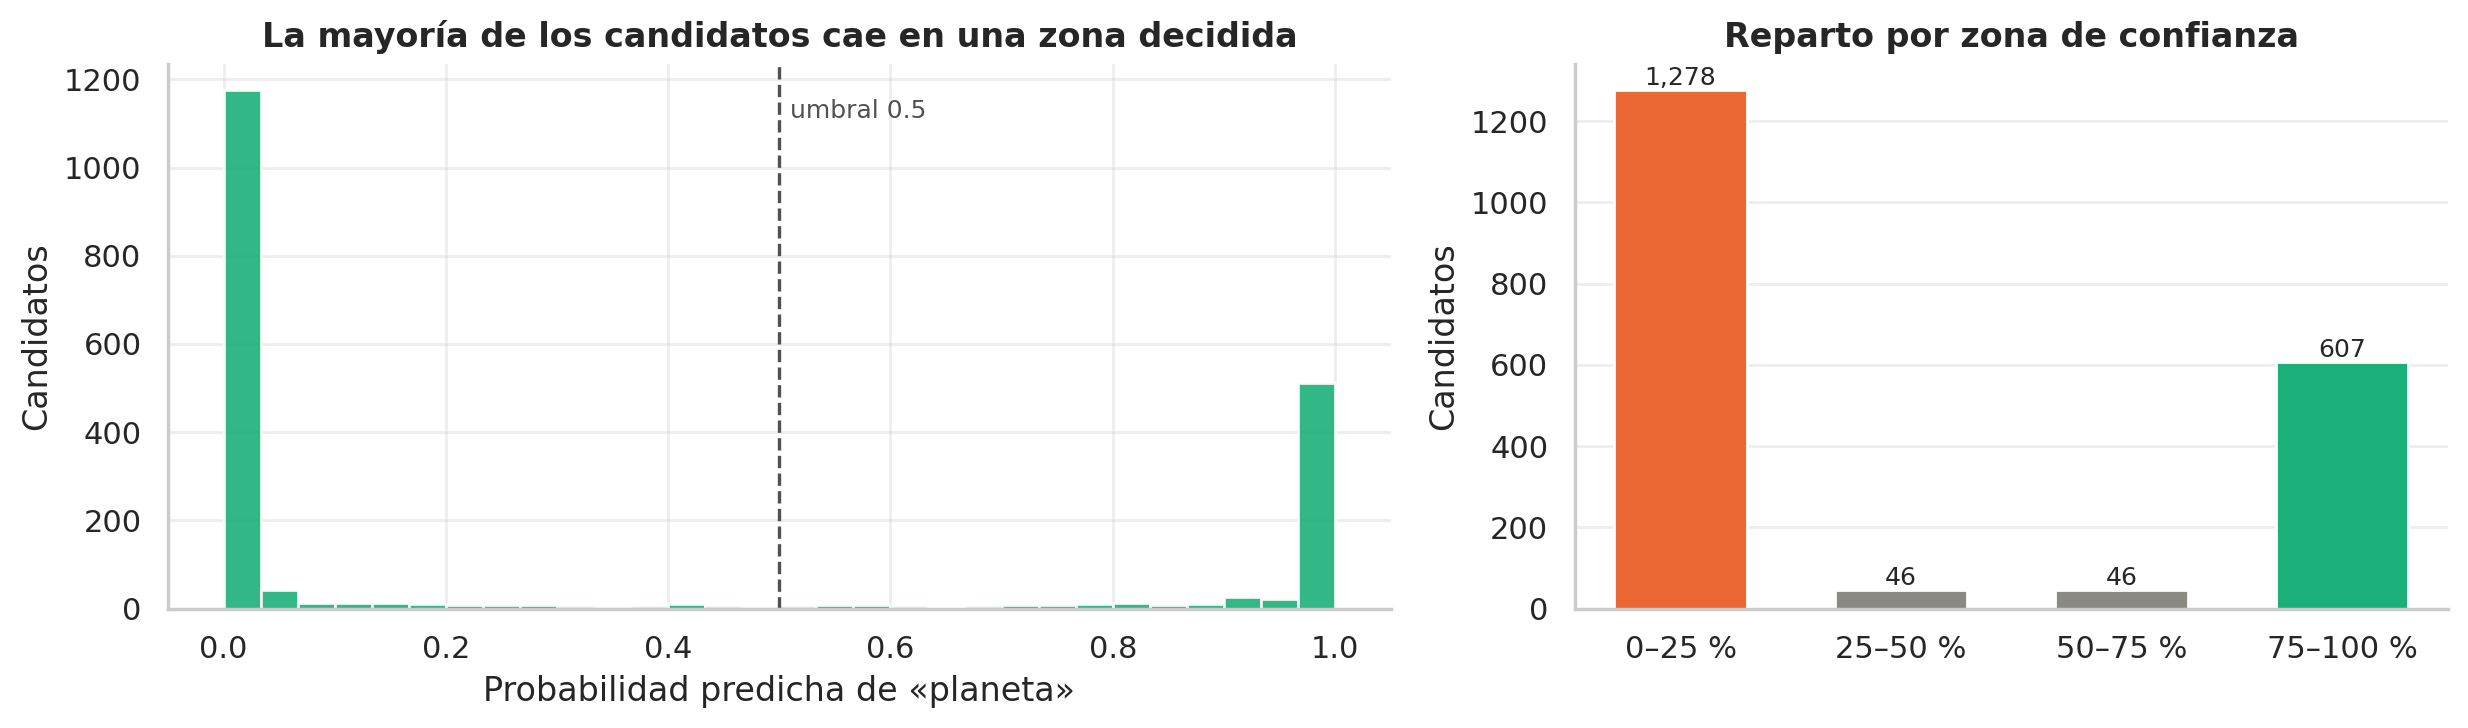
\includegraphics[width=\linewidth]{assets/images/fig-zonas.png}
    \caption{Probabilidades predichas y reparto por zonas de confianza}
    \label{fig:zonas}
    \par\medskip
    \begin{minipage}{\linewidth}
      \footnotesize\textit{Nota.} La línea discontinua es el umbral 0.5. La
      bimodalidad indica que el modelo no reparte la mitad de las decisiones cerca
      del azar.
    \end{minipage}
  \end{figure}

  La coherencia física del producto se verifica en dos planos
  (Figura~\ref{fig:mapa}). Primero, en el mapa periodo-radio, los 653 candidatos
  propuestos como planeta se apilan en la región de los planetas confirmados
  (radios entre Tierra y Neptuno, periodos intermedios) y no en la esquina de
  radio grande donde viven los eclipsamientos binarios. Segundo, en la
  multiplicidad: donde en realidad hay 81 \% de planetas (sistemas con dos o más
  señales), el modelo vota «planeta» para el 58 \% de los candidatos múltiples;
  donde solo hay 22 \% (una señal), vota para el 25 \%. El orden de las tasas es
  el correcto y el modelo lo aprendió sin que nadie le explicara la física; su
  prudencia frente a la tasa real (58 frente a 81) es coherente con un umbral
  conservador y con la incertidumbre propia de los candidatos.

  \begin{figure}[H]
    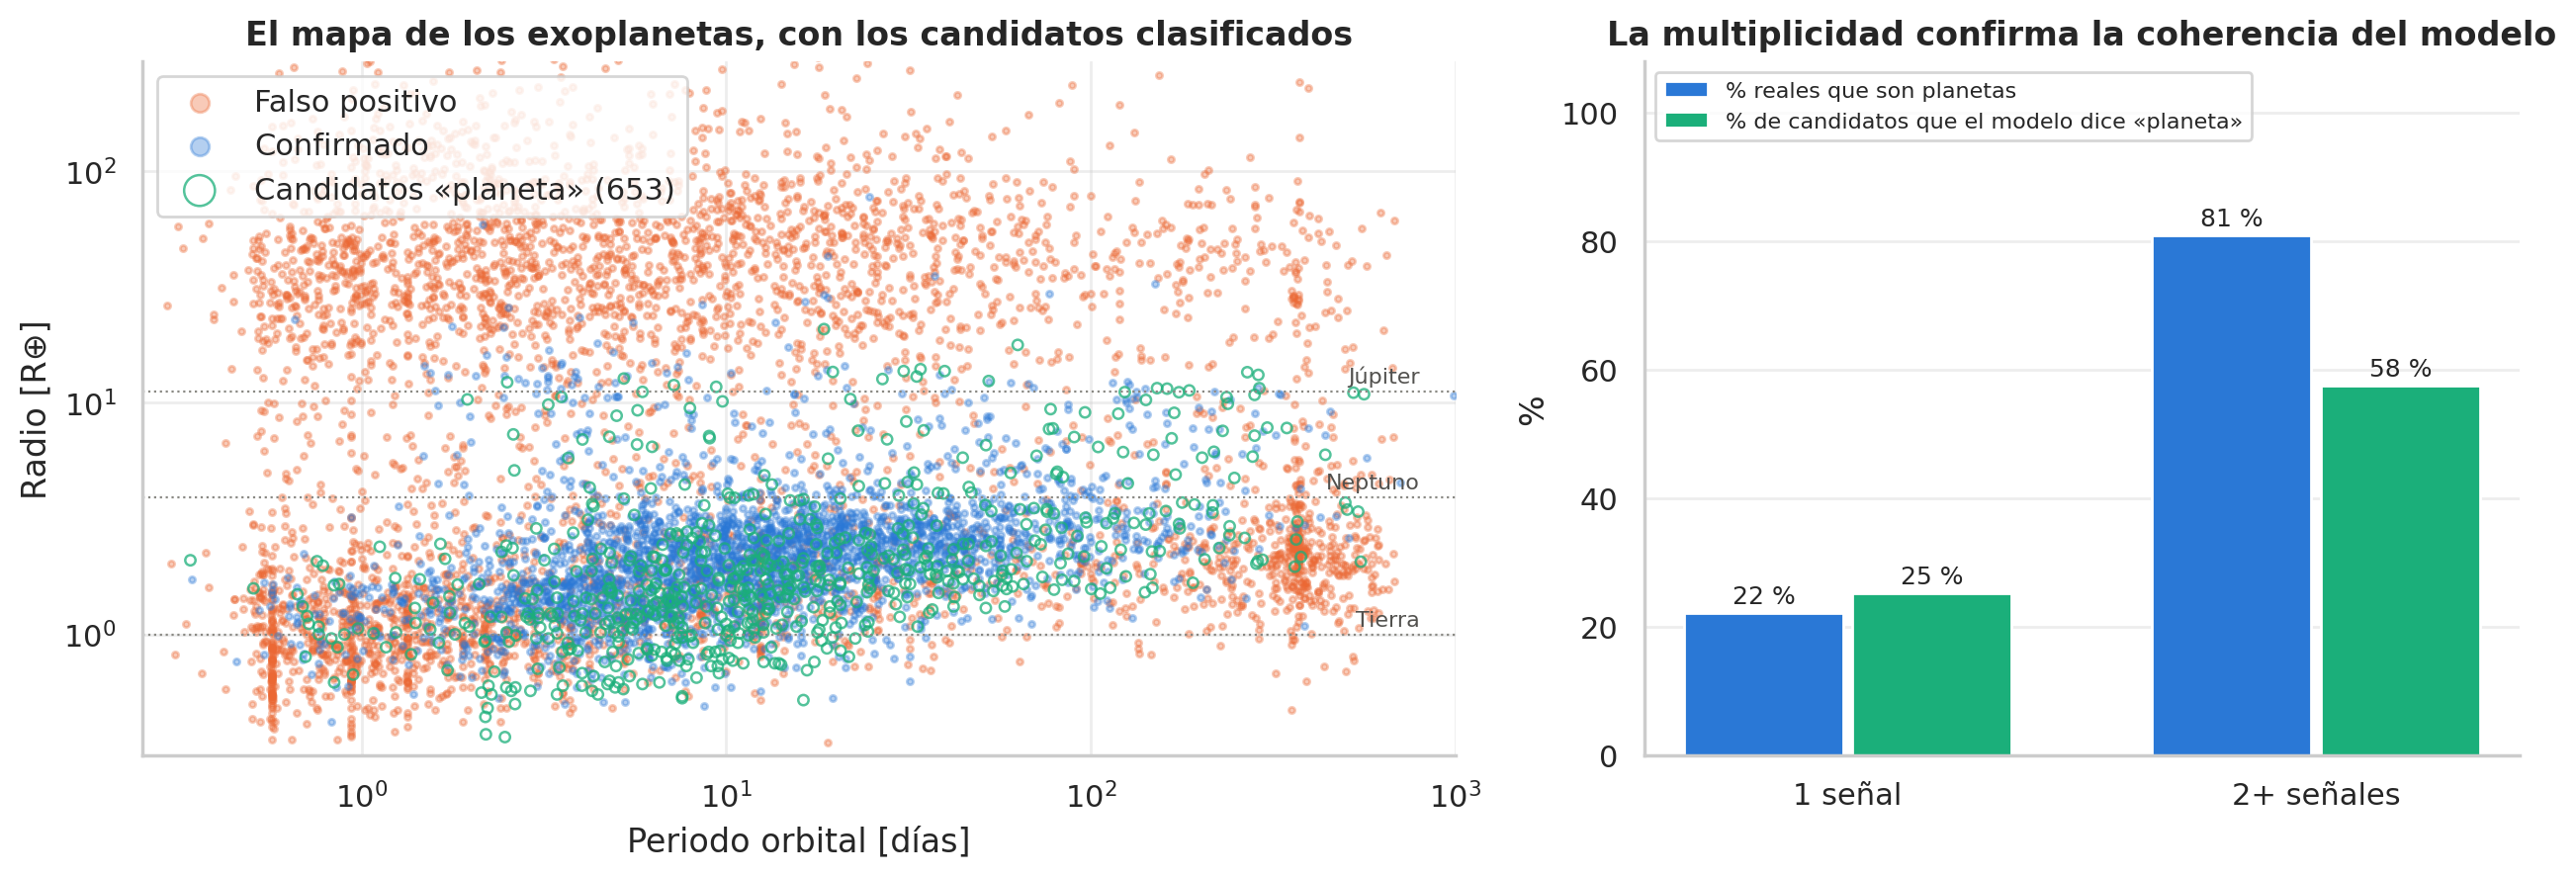
\includegraphics[width=\linewidth]{assets/images/fig-periodo-radio.png}
    \caption{Mapa periodo-radio con los candidatos clasificados y coherencia con la multiplicidad}
    \label{fig:mapa}
    \par\medskip
    \begin{minipage}{\linewidth}
      \footnotesize\textit{Nota.} Izquierda: los 653 candidatos propuestos como
      planeta (círculos verdes) sobre los KOI resueltos. Derecha: porcentaje de
      planetas reales y porcentaje de candidatos clasificados como planeta según
      la multiplicidad del sistema. Unión posicional por orden de filas entre
      candidatos y clasificados (sin clave estable, mismo orden de NB5).
    \end{minipage}
  \end{figure}

  La Tabla~\ref{tab:top10} muestra los diez primeros candidatos del ranking por
  probabilidad, todos con perfil físico atractivo: periodos de días a semanas,
  radios de super-Tierra a super-Tierra cálido y profundidades de tránsito bien
  medidas.

  \begin{table}[H]
    \caption{Diez primeros candidatos del ranking por probabilidad de planeta}
    \label{tab:top10}
    \begin{tabular}{@{}lccccc@{}}
      \toprule
      \# & KOI & Periodo (días) & Radio ($R_{\oplus}$) & Profundidad (ppm) & Probabilidad \\
      \midrule
      1 & K01145.01 & 30.59 & 2.32 & 465 & 1.000 \\
      2 & K04149.01 & 9.55 & 1.71 & 143 & 1.000 \\
      3 & K01338.02 & 42.04 & 1.66 & 267 & 1.000 \\
      4 & K02551.01 & 16.48 & 1.53 & 479 & 1.000 \\
      5 & K03396.01 & 36.26 & 1.82 & 380 & 1.000 \\
      6 & K01660.01 & 35.64 & 1.99 & 453 & 1.000 \\
      7 & K01628.03 & 37.84 & 1.76 & 233 & 1.000 \\
      8 & K01590.01 & 12.89 & 1.93 & 602 & 1.000 \\
      9 & K01573.02 & 7.14 & 1.38 & 222 & 1.000 \\
      10 & K03936.01 & 141.61 & 2.98 & 1 263 & 1.000 \\
      \bottomrule
    \end{tabular}
    \par\medskip
    \begin{minipage}{\linewidth}
      \footnotesize\textit{Nota.} Probabilidades redondeadas a tres decimales; los
      diez primeros superan 0.999. Periodo, radio y profundidad corresponden a los
      valores crudos del catálogo.
    \end{minipage}
  \end{table}

  \section{Discusión}

  El resultado principal del proyecto no es el número final sino la cadena que lo
  hace defendible. El mismo dataset que produce F1 macro de 0.983 produciría
  números perfectos e inútiles si se incluyeran las columnas de fuga: el modelo
  «sabría» el veredicto del vetting en lugar de estimarlo. Toda la ganancia del
  pipeline se construyó en la preparación, y la prueba tocada una sola vez
  garantiza que 0.983 es una estimación honesta del desempeño en candidatos
  nuevos. La jerarquía de importancia confirma que el modelo y el astrónomo
  miran lo mismo: calidad de la señal, eventos múltiples y geometría del
  tránsito \cite{thompson2018}, lo que da sustento a usarlo como sistema de
  priorización y no como caja negra.

  En la dirección de aplicación, el producto traduce la métrica a decisión
  operativa: una lista de 653 candidatos priorizada por probabilidad, con 607 en
  zona de alta confianza y 92 en zona de revisión manual. El reparto bimodal de la
  Figura~\ref{fig:zonas} y la coherencia con la multiplicidad
  (Figura~\ref{fig:mapa}) sugieren que las probabilidades del modelo son un buen
  resumen de la evidencia, aunque todavía no calibradas en sentido formal
  (véase la sección de trabajo futuro).

  \section{Limitaciones}

  Cuatro limitaciones acotan el alcance de los resultados. Primera, el modelo
  hereda la calidad de sus etiquetas: aprende de los veredictos del pipeline de
  vetting del catálogo \cite{thompson2018}, de modo que los errores sistemáticos
  del vetting (si los hay) se convierten en errores del modelo. Segunda, la
  muestra está condicionada por la sensibilidad de Kepler: el catálogo está
  sesgado hacia planetas de periodo corto y radio grande, así que el desempeño
  medido no es extrapolable tal cual a planetas tipo Tierra con años de periodo.
  Tercera, las probabilidades del gradient boosting no están calibradas: el
  umbral 0.5 se mantiene por simplicidad y comparabilidad con el baseline, pero
  para priorización estricta convendría calibrar (isotónica o Platt) y elegir el
  umbral según el coste relativo entre perder un planeta y hacer seguimiento
  inútil. Cuarta, el análisis de interpretabilidad se limita a importancia por
  permutación agregada; no captura interacciones ni direcciones parciales por
  clase.

  \section{Trabajo futuro}

  Las extensiones naturales del proyecto, en orden de valor: calibrar las
  probabilidades y optimizar el umbral con un coste explícito de los dos tipos de
  error; usar los 92 candidatos de zona gris como cola de \textit{active
  learning} para etiquetar ejemplos informativos con seguimiento real; modelar el
  sistema completo en lugar del KOI individual (el contexto de multiperiodicidad
  de la estrella es una señal que hoy solo entra de forma binaria); y empaquetar
  el producto en un dashboard interactivo para la sustentación, donde el tablero
  del NB5 (Figura~\ref{fig:tablero}) resume el panorama completo: el problema, el
  resultado, el método y la propuesta.

  \begin{figure}[H]
    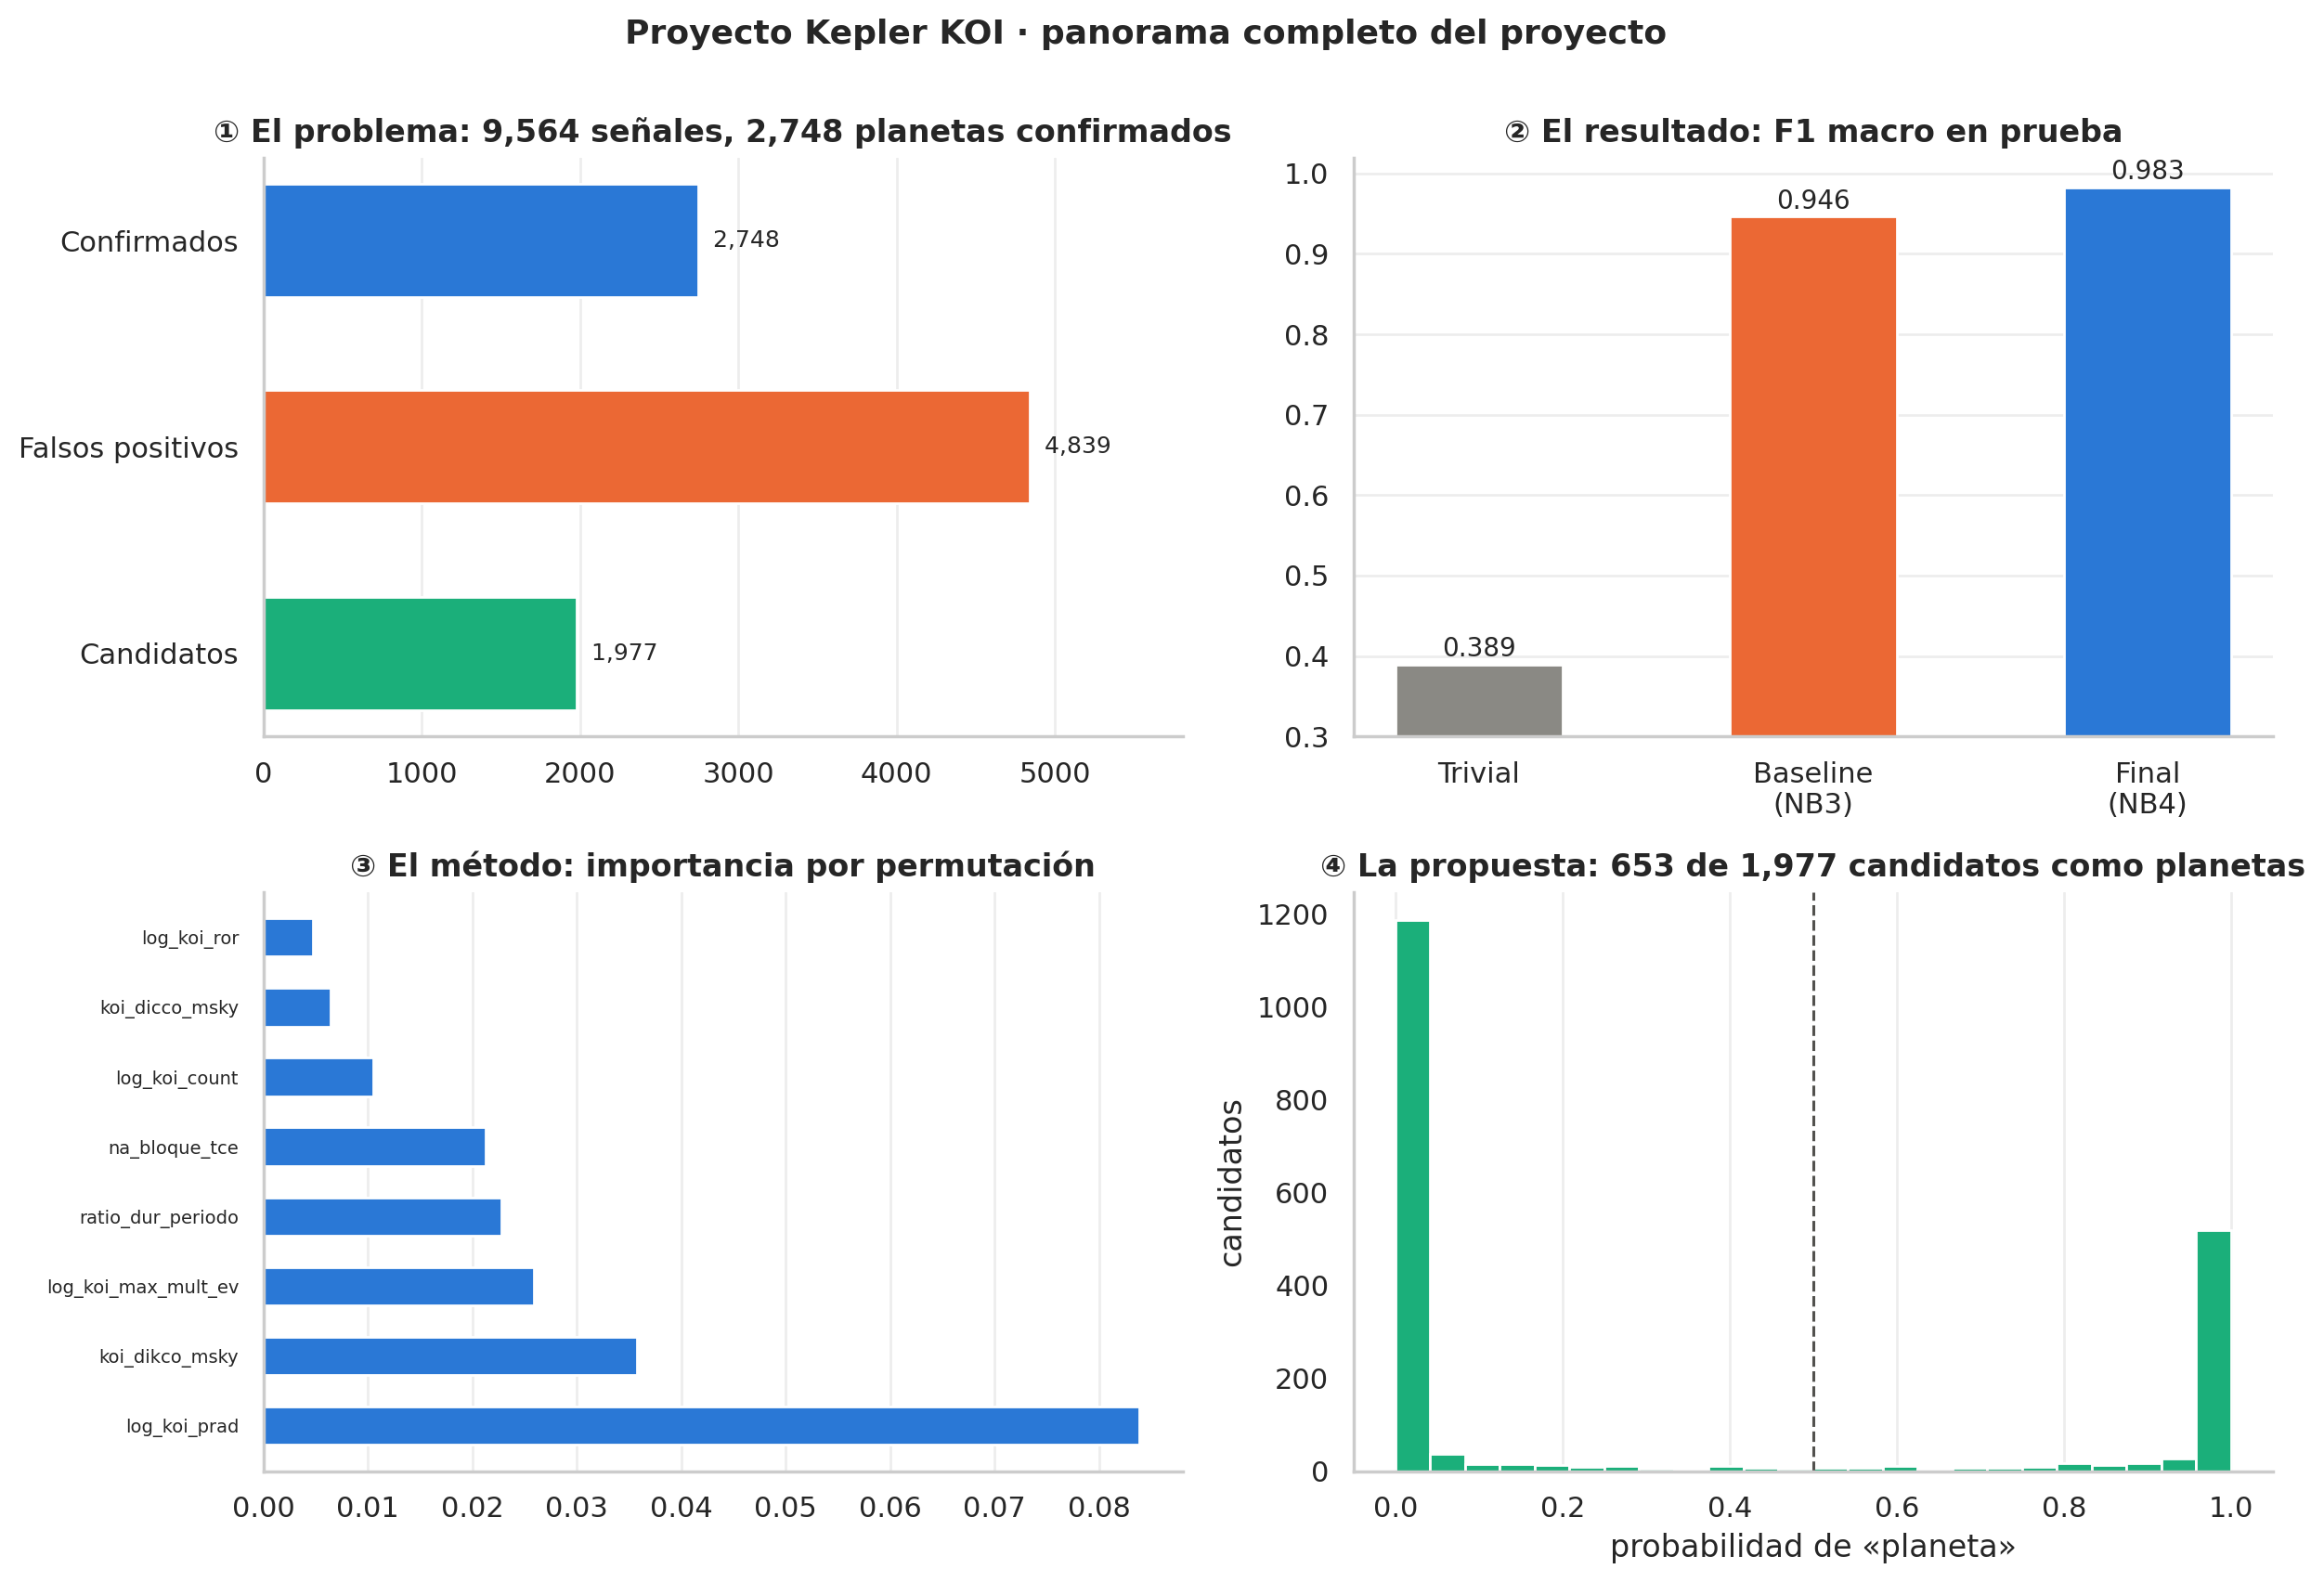
\includegraphics[width=\linewidth]{assets/images/fig-tablero.png}
    \caption{Tablero de resumen del proyecto para la sustentación}
    \label{fig:tablero}
    \par\medskip
    \begin{minipage}{\linewidth}
      \footnotesize\textit{Nota.} Cuatro paneles: composición del catálogo, F1
      macro en prueba, importancia por permutación y distribución de
      probabilidades de los candidatos.
    \end{minipage}
  \end{figure}

  \section{Conclusiones}

  El proyecto recorrió el ciclo completo de la ciencia de datos con disciplina de
  evaluación: exploración honesta, limpieza con control de fuga, partición fija,
  comparación justa de tres familias de modelos y una única evaluación final.
  El gradient boosting ganó con F1 macro de 0.983 y AUC de 0.997 en prueba,
  mejorando 0.037 al baseline lineal, con 98.0 \% de sensibilidad planetaria y
  solo 24 errores en 1 518 objetos. La importancia por permutación mostró que el
  modelo aprende física verificable, y el producto final convirtió ese desempeño
  en una lista priorizada de 653 candidatos a planeta sobre 1 977 sin verificar,
  con su probabilidad y su archivo reproducible. El repositorio entregado permite
  regenerar cada cifra de este informe ejecutando los cinco cuadernos en orden.

  \bibliographystyle{apa7cite}
  \bibliography{bib/references}

\end{document}
